\documentclass[12pt]{article}

\usepackage{amsmath,amsthm,amsfonts,amssymb,amsxtra}
\usepackage{tikz,array}
\usetikzlibrary{arrows}
\renewcommand{\theenumi}{(\alph{enumi})} 
\renewcommand{\labelenumi}{\theenumi}

\pagestyle{empty}
\setlength{\textwidth}{7in}
\setlength{\oddsidemargin}{-0.5in}
\setlength{\topmargin}{-1.0in}
\setlength{\textheight}{9.5in}

\theoremstyle{definition}
\newtheorem{problem}{Problem}

\begin{document}

\noindent{\large\bf MATH 242}\hfill{\large\bf Test \#4}\hfill{\large\bf
  Spring 2018}\hfill{\large\bf Page 1/8}\hrule

\bigskip
\begin{center}
  \begin{tabular}{|ll|}
    \hline & \cr
    {\bf Name: } & \makebox[12cm]{\hrulefill}\cr & \cr
    {\bf VIP ID:} & \makebox[12cm]{\hrulefill}\cr & \cr
    \hline
  \end{tabular}
\end{center}
\begin{itemize}
\item Write your name and your VIP ID in the space provided above.
\item The test has eight (8) pages, including this one and one page of scratch paper at the end with a table of Laplace transforms.
\item \textbf{Do not answer} any problem in the scratch paper.  All solutions must be provided on pages 2--7 where it proceeds.
\item Show sufficient work to justify all answers unless otherwise stated in the problem.  Correct answers with inconsistent work may not be given credit.
\item Credit for each problem is given at the right of each problem
  number. 
\end{itemize}
\hrule

\begin{center}
  \begin{tabular}{|c|c|c|}
    \hline
    &&\cr
    {\large\bf Page} & {\large\bf Max} & {\large\bf Points} \cr
    &&\cr
    \hline
    &&\cr
    {\Large 2} & \Large 15 & \cr
    &&\cr
    \hline
    &&\cr
    {\Large 3} & \Large 15 & \cr
    &&\cr
    \hline
    &&\cr
    {\Large 4} & \Large 20 & \cr
    &&\cr
    \hline
    &&\cr
    {\Large 5} & \Large 20 & \cr
    &&\cr
    \hline
    &&\cr
    {\Large 6} & \Large 10 & \cr
    &&\cr
    \hline
    &&\cr
    {\Large 7} & \Large 20 & \cr
    &&\cr
    \hline\hline
    &&\cr
    {\large\bf Total} & \Large 100 & \cr
    &&\cr
    \hline
  \end{tabular}
\end{center}
\newpage

%%%%%%%%%%%%%%%%%%%%%%%%%%%%%%%%%%%%% Page 2
\noindent{\large\bf MATH 242}\hfill{\large\bf Test \#4}\hfill{\large\bf Spring 2018}\hfill{\large\bf Page 2/8}\hrule

\bigskip
\begin{problem}[15 pts---5 pts each part]
A body with mass 0.5~kg is attached to the end of a spring that is stretched 2~m by a force of 10~N.  It is set in motion one meter to the right, and moving to the left at that time with an initial velocity of 5~m/s.
\begin{enumerate}
  \item Find the position function of the body.
  \vspace{4cm}
  \begin{flushright}
  \begin{tikzpicture}
  \draw (-0.75cm, 0.5cm) node{$x(t)=$};
  \draw (0cm,-0.2cm) rectangle (5cm,1.2cm);
  \end{tikzpicture}
  \end{flushright}
  \item Indicate the amplitude, frequency, period of oscillation and time lag of this motion.
  \vspace{4cm}
  \begin{flushright}
  \begin{tikzpicture}
  \draw (-1.2cm, 0.5cm) node{Amplitude:};
  \draw (0cm,-0.2cm) rectangle (2cm,1.2cm);
  \begin{scope}[xshift=4.5cm]
  \draw (-1.2cm, 0.5cm) node{Frequency:};
  \draw (0cm,-0.2cm) rectangle (2cm,1.2cm);
  \end{scope}
  \begin{scope}[xshift=8.5cm]
  \draw (-1cm, 0.5cm) node{Period:};
  \draw (0cm,-0.2cm) rectangle (2cm,1.2cm);
  \end{scope}
  \begin{scope}[xshift=13cm]
  \draw (-1cm, 0.5cm) node{Time lag:};
  \draw (0cm,-0.2cm) rectangle (2cm,1.2cm);
  \end{scope}
  \end{tikzpicture}
  \end{flushright}
  \item Sketch the solution curve.  Make sure to label all relevant information (amplitude, time lag and period).
\end{enumerate}
\end{problem} 

\newpage

%%%%%%%%%%%%%%%%%%%%%%%%%%%%%%%%%%%%% Page 3
\noindent{\large\bf MATH 242}\hfill{\large\bf Test \#4}\hfill{\large\bf
  Spring 2018}\hfill{\large\bf Page 3/8}\hrule

\bigskip
\begin{problem}[15 pts---5 pts each part]
The mass and spring of the previous problem are now attached also to a dashpot that provides 1~N of resistance for each meter per second of velocity.  The mass is set in motion with the same initial position and initial velocity as before.
\begin{enumerate}
  \item Find the position function of the body.
  \vspace{4cm}
  \begin{flushright}
  \begin{tikzpicture}
  \draw (-0.75cm, 0.5cm) node{$x(t)=$};
  \draw (0cm,-0.2cm) rectangle (5cm,1.2cm);
  \end{tikzpicture}
  \end{flushright}
  \item Indicate the amplitude, the new frequency, pseudoperiod and new time lag of this motion.
  \vspace{4cm}
  \begin{flushright}
  \begin{tikzpicture}
  \draw (-1.2cm, 0.5cm) node{Amplitude:};
  \draw (0cm,-0.2cm) rectangle (2cm,1.2cm);
  \begin{scope}[xshift=4.4cm]
  \draw (-1.2cm, 0.5cm) node{Frequency:};
  \draw (0cm,-0.2cm) rectangle (2cm,1.2cm);
  \end{scope}
  \begin{scope}[xshift=9.3cm]
  \draw (-1.4cm, 0.5cm) node{Pseudoperiod:};
  \draw (0cm,-0.2cm) rectangle (2cm,1.2cm);
  \end{scope}
  \begin{scope}[xshift=13.5cm]
  \draw (-1cm, 0.5cm) node{Time lag:};
  \draw (0cm,-0.2cm) rectangle (2cm,1.2cm);
  \end{scope}
  \end{tikzpicture}
  \end{flushright}
  \item Sketch the solution curve.  Make sure to label all relevant information (amplitude, time lag and pseudoperiod).
\end{enumerate}
\end{problem} 

\newpage

%%%%%%%%%%%%%%%%%%%%%%%%%%%%%%%%%%%%% Page 4
\noindent{\large\bf MATH 242}\hfill{\large\bf Test \#4}\hfill{\large\bf
  Spring 2018}\hfill{\large\bf Page 4/8}\hrule

\bigskip
\begin{problem}[20 pts---10 pts each part]
Suppose that the mass in a mass-spring-dashpot system with $m=10$, $c=9$ and $k=2$ is set in motion with $x(0)=0$ and $x'(0)=-5$.
\begin{enumerate}
  \item Find the position function of the body.
  \vspace{4cm}
  \begin{flushright}
  \begin{tikzpicture}
  \draw (-0.75cm, 0.5cm) node{$x(t)=$};
  \draw (0cm,-0.2cm) rectangle (5cm,1.2cm);
  \end{tikzpicture}
  \end{flushright}
  \item Sketch the solution curve for $t \in [0, 20]$.  Indicate clearly how far the mass moves to the left before starting back toward the origin (show all necessary work to find this value)
\end{enumerate}
\end{problem}
\newpage

%%%%%%%%%%%%%%%%%%%%%%%%%%%%%%%%%%%%% Page 5
\noindent{\large\bf MATH 242}\hfill{\large\bf Test \#4}\hfill{\large\bf
  Spring 2018}\hfill{\large\bf Page 5/8}\hrule

\bigskip
\begin{problem}[20 pts---10 pts each]
Consider an undamped forced motion with equation 
\begin{equation*}
x''+9x=-64\cos 5t.
\end{equation*}
\begin{enumerate}
  \item Assume $m=1$.  Find the values of $k$, $F_0$ and $\omega$.
  \begin{flushright}
  \begin{tikzpicture}
  \draw (-0.5cm, 0.5cm) node{$k=$};
  \draw (0cm,-0.2cm) rectangle (2cm,1.2cm);
  \begin{scope}[xshift=4cm]
  \draw (-0.5cm, 0.5cm) node{$F_0=$};
  \draw (0cm,-0.2cm) rectangle (2cm,1.2cm);
  \end{scope}
  \begin{scope}[xshift=8cm]
  \draw (-0.5cm, 0.5cm) node{$\omega=$};
  \draw (0cm,-0.2cm) rectangle (2cm,1.2cm);
  \end{scope}
  \end{tikzpicture}
  \end{flushright}
  \item Find $x(t)$ if $x(0)=x'(0)=0$.  Sketch the motion for $t \in [0,2\pi]$. 
  \vspace{16cm}
  \begin{flushright}
  \begin{tikzpicture}
  \draw (-0.75cm, 0.5cm) node{$x(t)=$};
  \draw (0cm,-0.2cm) rectangle (5cm,1.2cm);
  \end{tikzpicture}
  \end{flushright}
\end{enumerate}
\end{problem}
\newpage

%%%%%%%%%%%%%%%%%%%%%%%%%%%%%%%%%%%%% Page 6
\noindent{\large\bf MATH 242}\hfill{\large\bf Test \#4}\hfill{\large\bf
  Spring 2018}\hfill{\large\bf Page 6/8}\hrule

\bigskip
\begin{problem}[10 pts]
Consider a damped forced motion with equation 
\begin{equation*}
x'' + 2x' + 9x = 10\cos 4t.
\end{equation*}
Find $x(t)$ if $x(0)=x'(0)=0$.  Sketch the motion for $t \in [0,2\pi]$.
  \vspace{18cm}
  \begin{flushright}
  \begin{tikzpicture}
  \draw (-0.75cm, 0.5cm) node{$x(t)=$};
  \draw (0cm,-0.2cm) rectangle (5cm,1.2cm);
  \end{tikzpicture}
  \end{flushright}
\end{problem}
\newpage

%%%%%%%%%%%%%%%%%%%%%%%%%%%%%%%%%%%%% Page 7
\noindent{\large\bf MATH 242}\hfill{\large\bf Test \#4}\hfill{\large\bf
  Spring 2018}\hfill{\large\bf Page 7/8}\hrule

\bigskip
\begin{problem}[20 pts---10 pts each]
Consider an undamped forced motion with equation 
\begin{equation*}
x''+25x=35\cos 5t.
\end{equation*}
\begin{enumerate}
  \item Assume $m=1$.  Find the values of $k$, $F_0$ and $\omega$.
  \begin{flushright}
  \begin{tikzpicture}
  \draw (-0.5cm, 0.5cm) node{$k=$};
  \draw (0cm,-0.2cm) rectangle (2cm,1.2cm);
  \begin{scope}[xshift=4cm]
  \draw (-0.5cm, 0.5cm) node{$F_0=$};
  \draw (0cm,-0.2cm) rectangle (2cm,1.2cm);
  \end{scope}
  \begin{scope}[xshift=8cm]
  \draw (-0.5cm, 0.5cm) node{$\omega=$};
  \draw (0cm,-0.2cm) rectangle (2cm,1.2cm);
  \end{scope}
  \end{tikzpicture}
  \end{flushright}
  \item Find $x(t)$ if $x(0)=x'(0)=0$.  Sketch the motion for $t \in [0,2\pi]$.
  \vspace{16cm}
  \begin{flushright}
  \begin{tikzpicture}
  \draw (-0.75cm, 0.5cm) node{$x(t)=$};
  \draw (0cm,-0.2cm) rectangle (5cm,1.2cm);
  \end{tikzpicture}
  \end{flushright}
\end{enumerate}
\end{problem}
\newpage

%%%%%%%%%%%%%%%%%%%%%%%%%%%%%%%%%%%%% Page 8
\noindent{\large\bf MATH 242}\hfill{\large\bf Test \#4}\hfill{\large\bf
  Spring 2018}\hfill{\large\bf Page 8/8}\hrule

\bigskip
\begin{center}
%\includegraphics[width=\linewidth]{table.pdf}
\begin{tikzpicture}
  \node[scale=0.97]{
 \begin{tabular}{|m{1.2cm}|m{4.3cm}l||m{2.1cm}|m{4.3cm}l|}
 \hline
    $f(x)$\raisebox{0.5cm} & $\mathcal{L}\{f\}=\int_0^\infty e^{-sx}f(x)\, dx$\raisebox{0.5cm} & &
    \raisebox{0.5cm} & \raisebox{0.5cm} & \\[0.4cm] 
    \hline \hline
    $1$ & $\dfrac{1}{s}$\raisebox{0.6cm} & $s>0$ &
    $cf(x)\pm g(x)$ & $cF(s) \pm G(s)$\raisebox{0.4cm} & $s>max(a,b)$ \\[0.4cm]
    \hline
    $x^n$ & $\dfrac{n!}{s^{n+1}}$\raisebox{0.6cm} & $s>0$ & $e^{\alpha x}f(x)$ & $F(s-\alpha)$\raisebox{0.4cm} & $s>a+\alpha$ \\[0.4cm]
    \hline
    $e^{\alpha x}$ & $\dfrac{1}{s-\alpha}$\raisebox{0.6cm} & $s>\alpha$ &
    $x^n f(x)$ & $(-1)^n F^{(n)}(s)$\raisebox{0.4cm} & $s>a$ \\[0.4cm]
    \hline
    $\sin \beta x$ & $\dfrac{\beta}{s^2+\beta^2}$\raisebox{0.6cm} & $s>0$ & $f'(x)$ & $s F(s) -f(0)$\raisebox{0.4cm} & \\[0.4cm]
    \hline
    $\cos \beta x$ & $\dfrac{s}{s^2+\beta^2}$\raisebox{0.6cm} & $s>0$ &$f''(x)$\raisebox{0.4cm} & $s^2F(s) - sf(0)  - f'(0)$ & \\[0.4cm]
    \hline
    \end{tabular} };
    \end{tikzpicture}
\end{center}

\end{document}
